\documentclass[../labs.tex]{subfiles}

\pagestyle{main}
\renewcommand{\leftmark}{Lab Report \thesection}

\begin{document}




\noindent Steven Labalme\\
12 January 2023\hfill
26 January 2023

\section{UV-VIS ANALYSIS OF IODINE}
\begin{figure}[H]
    \centering
    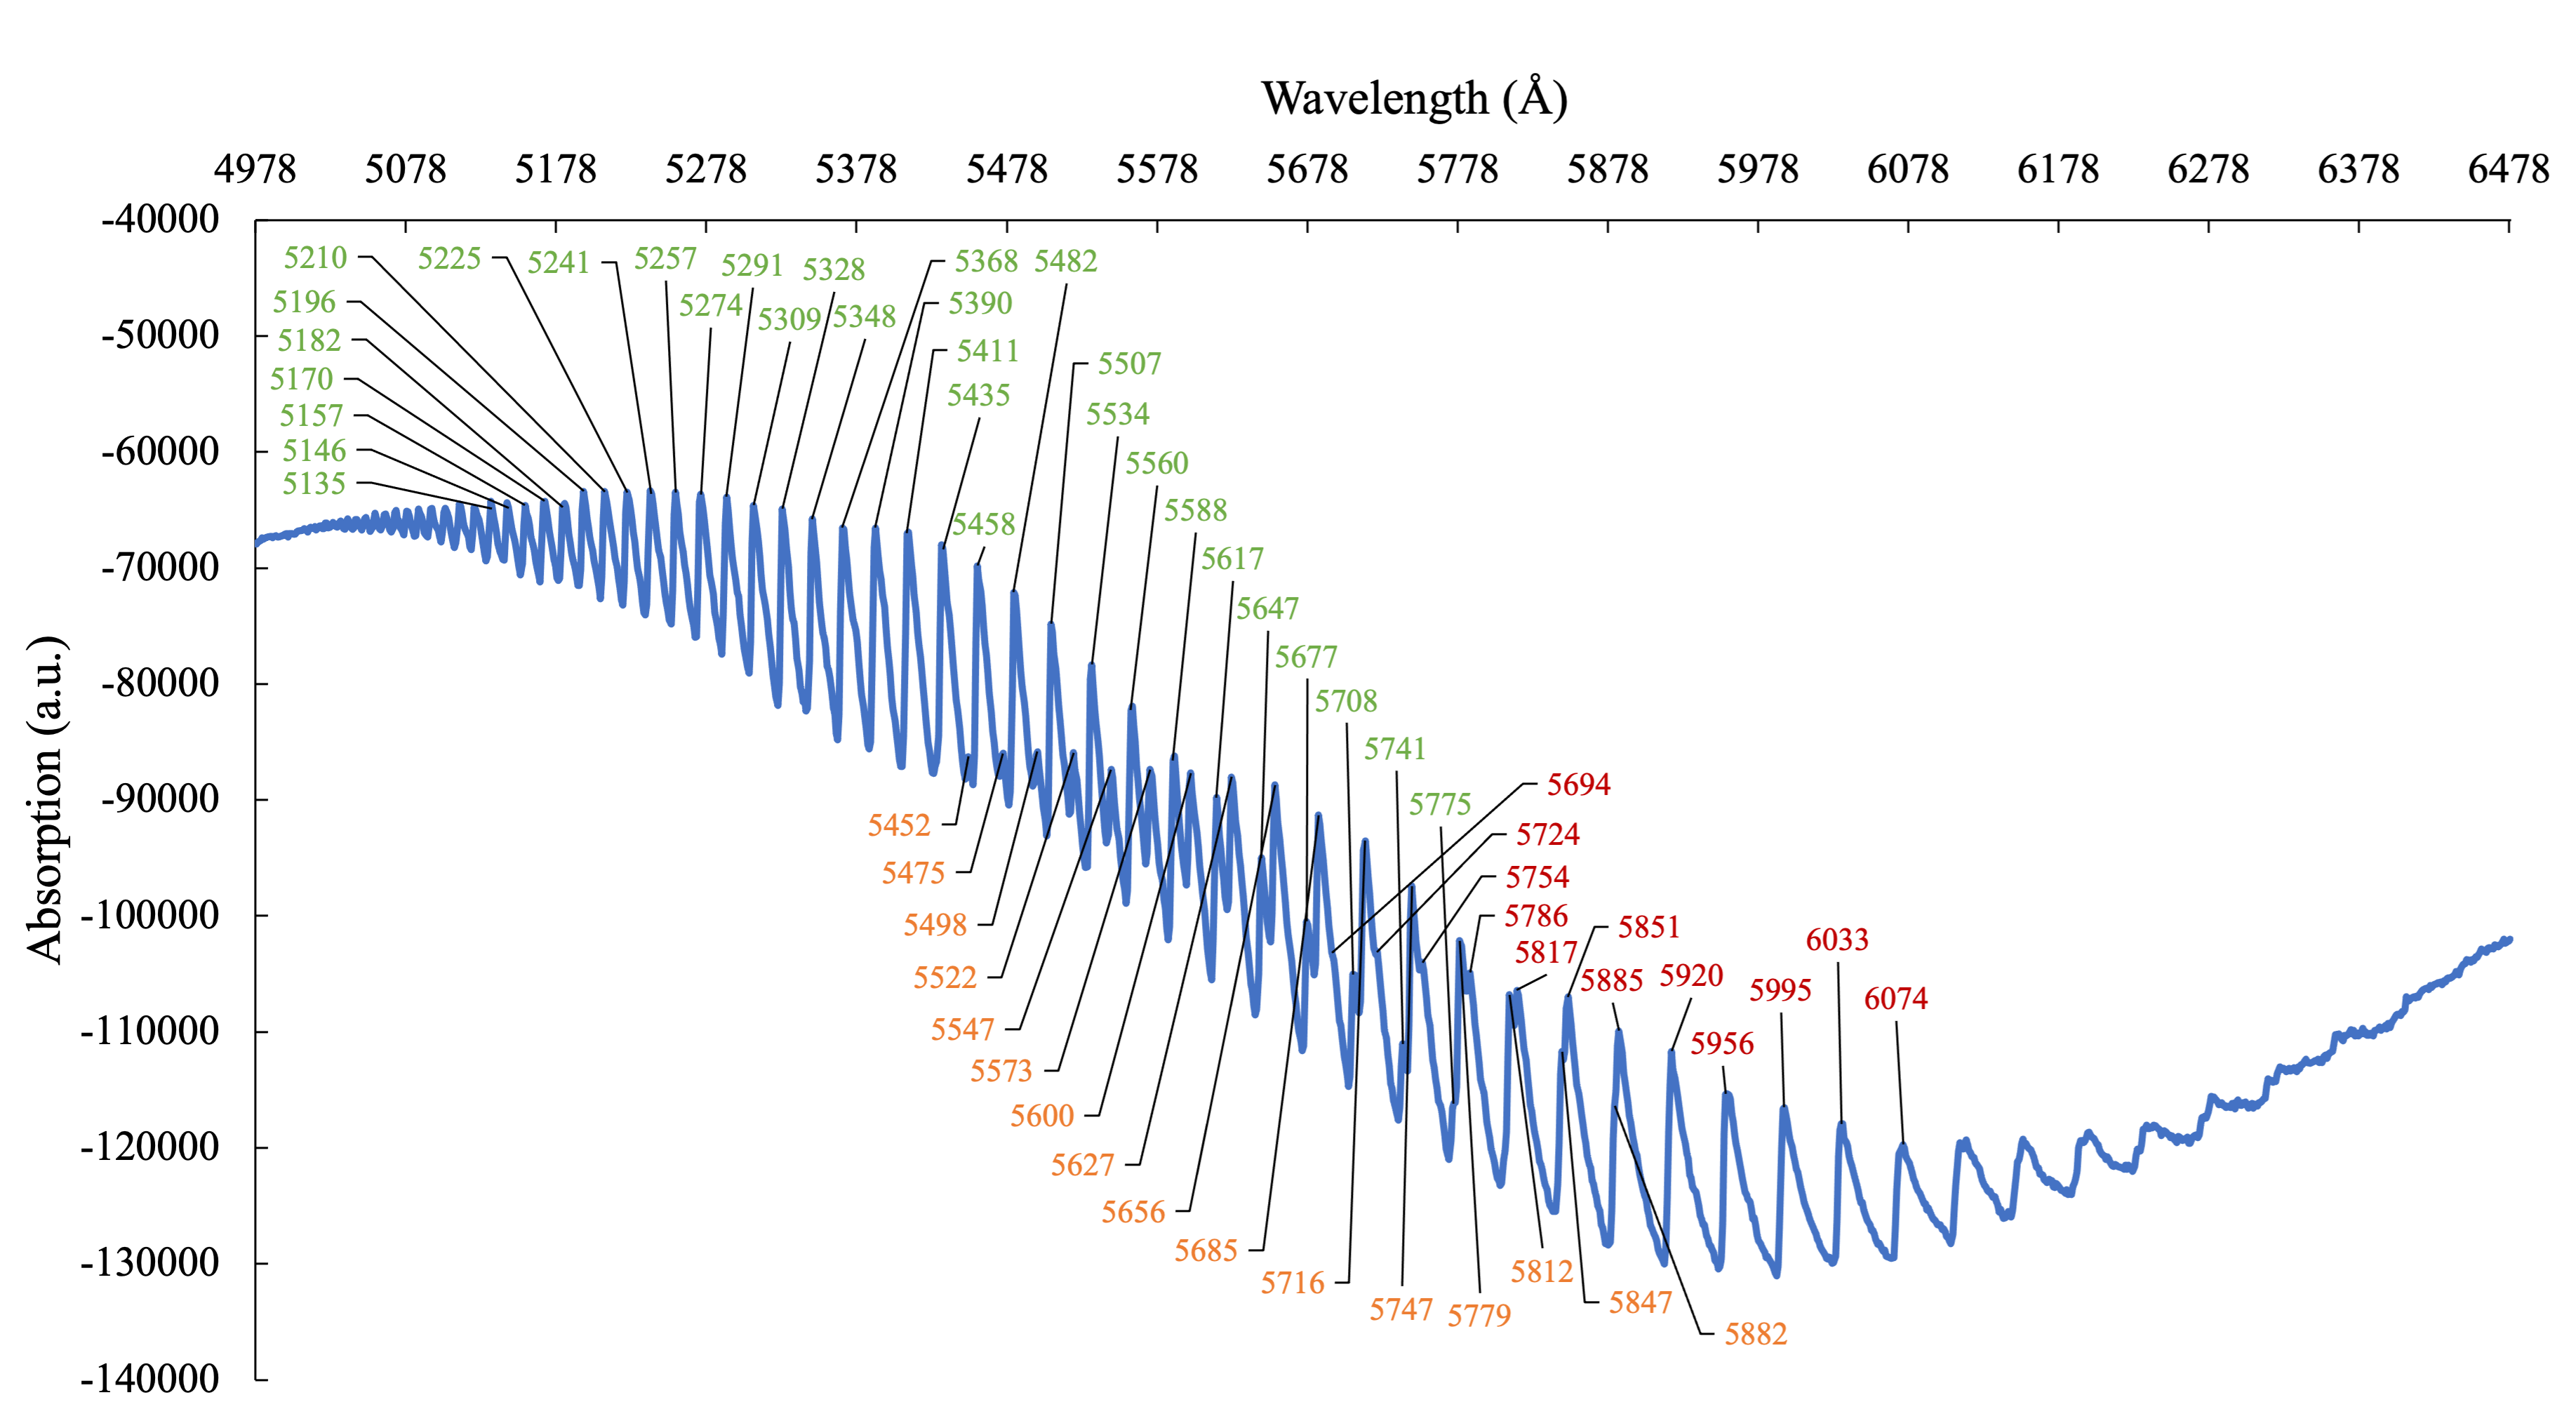
\includegraphics[width=0.95\linewidth]{lab1-I2Spectrum.png}
    \caption{The absorption spectrum of gaseous \ce{I2} between $\lambda=\SIrange{5000}{6500}{\angstrom}$.}
    \label{fig:I2Spectrum}
\end{figure}

\begin{table}[H]
    \centering
    \small
    \renewcommand{\arraystretch}{1.2}
    \begin{tabular}{|c|c|c|c|c|c|c|c|c|}
        \hline
        $\bm{v'}$ & $\bm{v''}$ & $\bm{\omega\ (\textbf{cm}^{-1})}$ & $\bm{v'}$ & $\bm{v''}$ & $\bm{\omega\ (\textbf{cm}^{-1})}$ & $\bm{v'}$ & $\bm{v''}$ & $\bm{\omega\ (\textbf{cm}^{-1})}$\\
        \hline
           &   &       &    &   &       & 10 & 2 & 16463\\ \hline
           &   &       &    &   &       & 11 & 2 & 16575\\ \hline
           &   &       &    &   &       & 12 & 2 & 16680\\ \hline
           &   &       & 13 & 1 & 17001 & 13 & 2 & 16789\\ \hline
        14 & 0 & 17316 & 14 & 1 & 17102 & 14 & 2 & 16891\\ \hline
        15 & 0 & 17418 & 15 & 1 & 17205 & 15 & 2 & 16992\\ \hline
        16 & 0 & 17519 & 16 & 1 & 17304 & 16 & 2 & 17091\\ \hline
        17 & 0 & 17614 & 17 & 1 & 17400 & 17 & 2 & 17190\\ \hline
        18 & 0 & 17708 & 18 & 1 & 17494 & 18 & 2 & 17283\\ \hline
        19 & 0 & 17803 & 19 & 1 & 17590 & 19 & 2 & 17379\\ \hline
        20 & 0 & 17895 & 20 & 1 & 17680 & 20 & 2 & 17470\\ \hline
        21 & 0 & 17985 & 21 & 1 & 17771 & 21 & 2 & 17562\\ \hline
        22 & 0 & 18070 & 22 & 1 & 17857 &    &   &      \\ \hline
        23 & 0 & 18158 & 23 & 1 & 17943 &    &   &      \\ \hline
        24 & 0 & 18241 & 24 & 1 & 18027 &    &   &      \\ \hline
        25 & 0 & 18321 & 25 & 1 & 18109 &    &   &      \\ \hline
        26 & 0 & 18399 & 26 & 1 & 18188 &    &   &      \\ \hline
        27 & 0 & 18480 & 27 & 1 & 18264 &    &   &      \\ \hline
        28 & 0 & 18552 & 28 & 1 & 18341 &    &   &      \\ \hline
        29 & 0 & 18628 &    &   &       &    &   &      \\ \hline
        30 & 0 & 18698 &    &   &       &    &   &      \\ \hline
        31 & 0 & 18768 &    &   &       &    &   &      \\ \hline
        32 & 0 & 18835 &    &   &       &    &   &      \\ \hline
        33 & 0 & 18900 &    &   &       &    &   &      \\ \hline
        34 & 0 & 18960 &    &   &       &    &   &      \\ \hline
        35 & 0 & 19022 &    &   &       &    &   &      \\ \hline
        36 & 0 & 19080 &    &   &       &    &   &      \\ \hline
        37 & 0 & 19138 &    &   &       &    &   &      \\ \hline
        38 & 0 & 19193 &    &   &       &    &   &      \\ \hline
        39 & 0 & 19245 &    &   &       &    &   &      \\ \hline
        40 & 0 & 19297 &    &   &       &    &   &      \\ \hline
        41 & 0 & 19342 &    &   &       &    &   &      \\ \hline
        42 & 0 & 19391 &    &   &       &    &   &      \\ \hline
        43 & 0 & 19432 &    &   &       &    &   &      \\ \hline
        44 & 0 & 19474 &    &   &       &    &   &      \\ \hline
    \end{tabular}
    \caption{Peaks and their corresponding transitions.}
    \label{tab:peakTransition}
\end{table}

\begin{figure}[H]
    \centering
    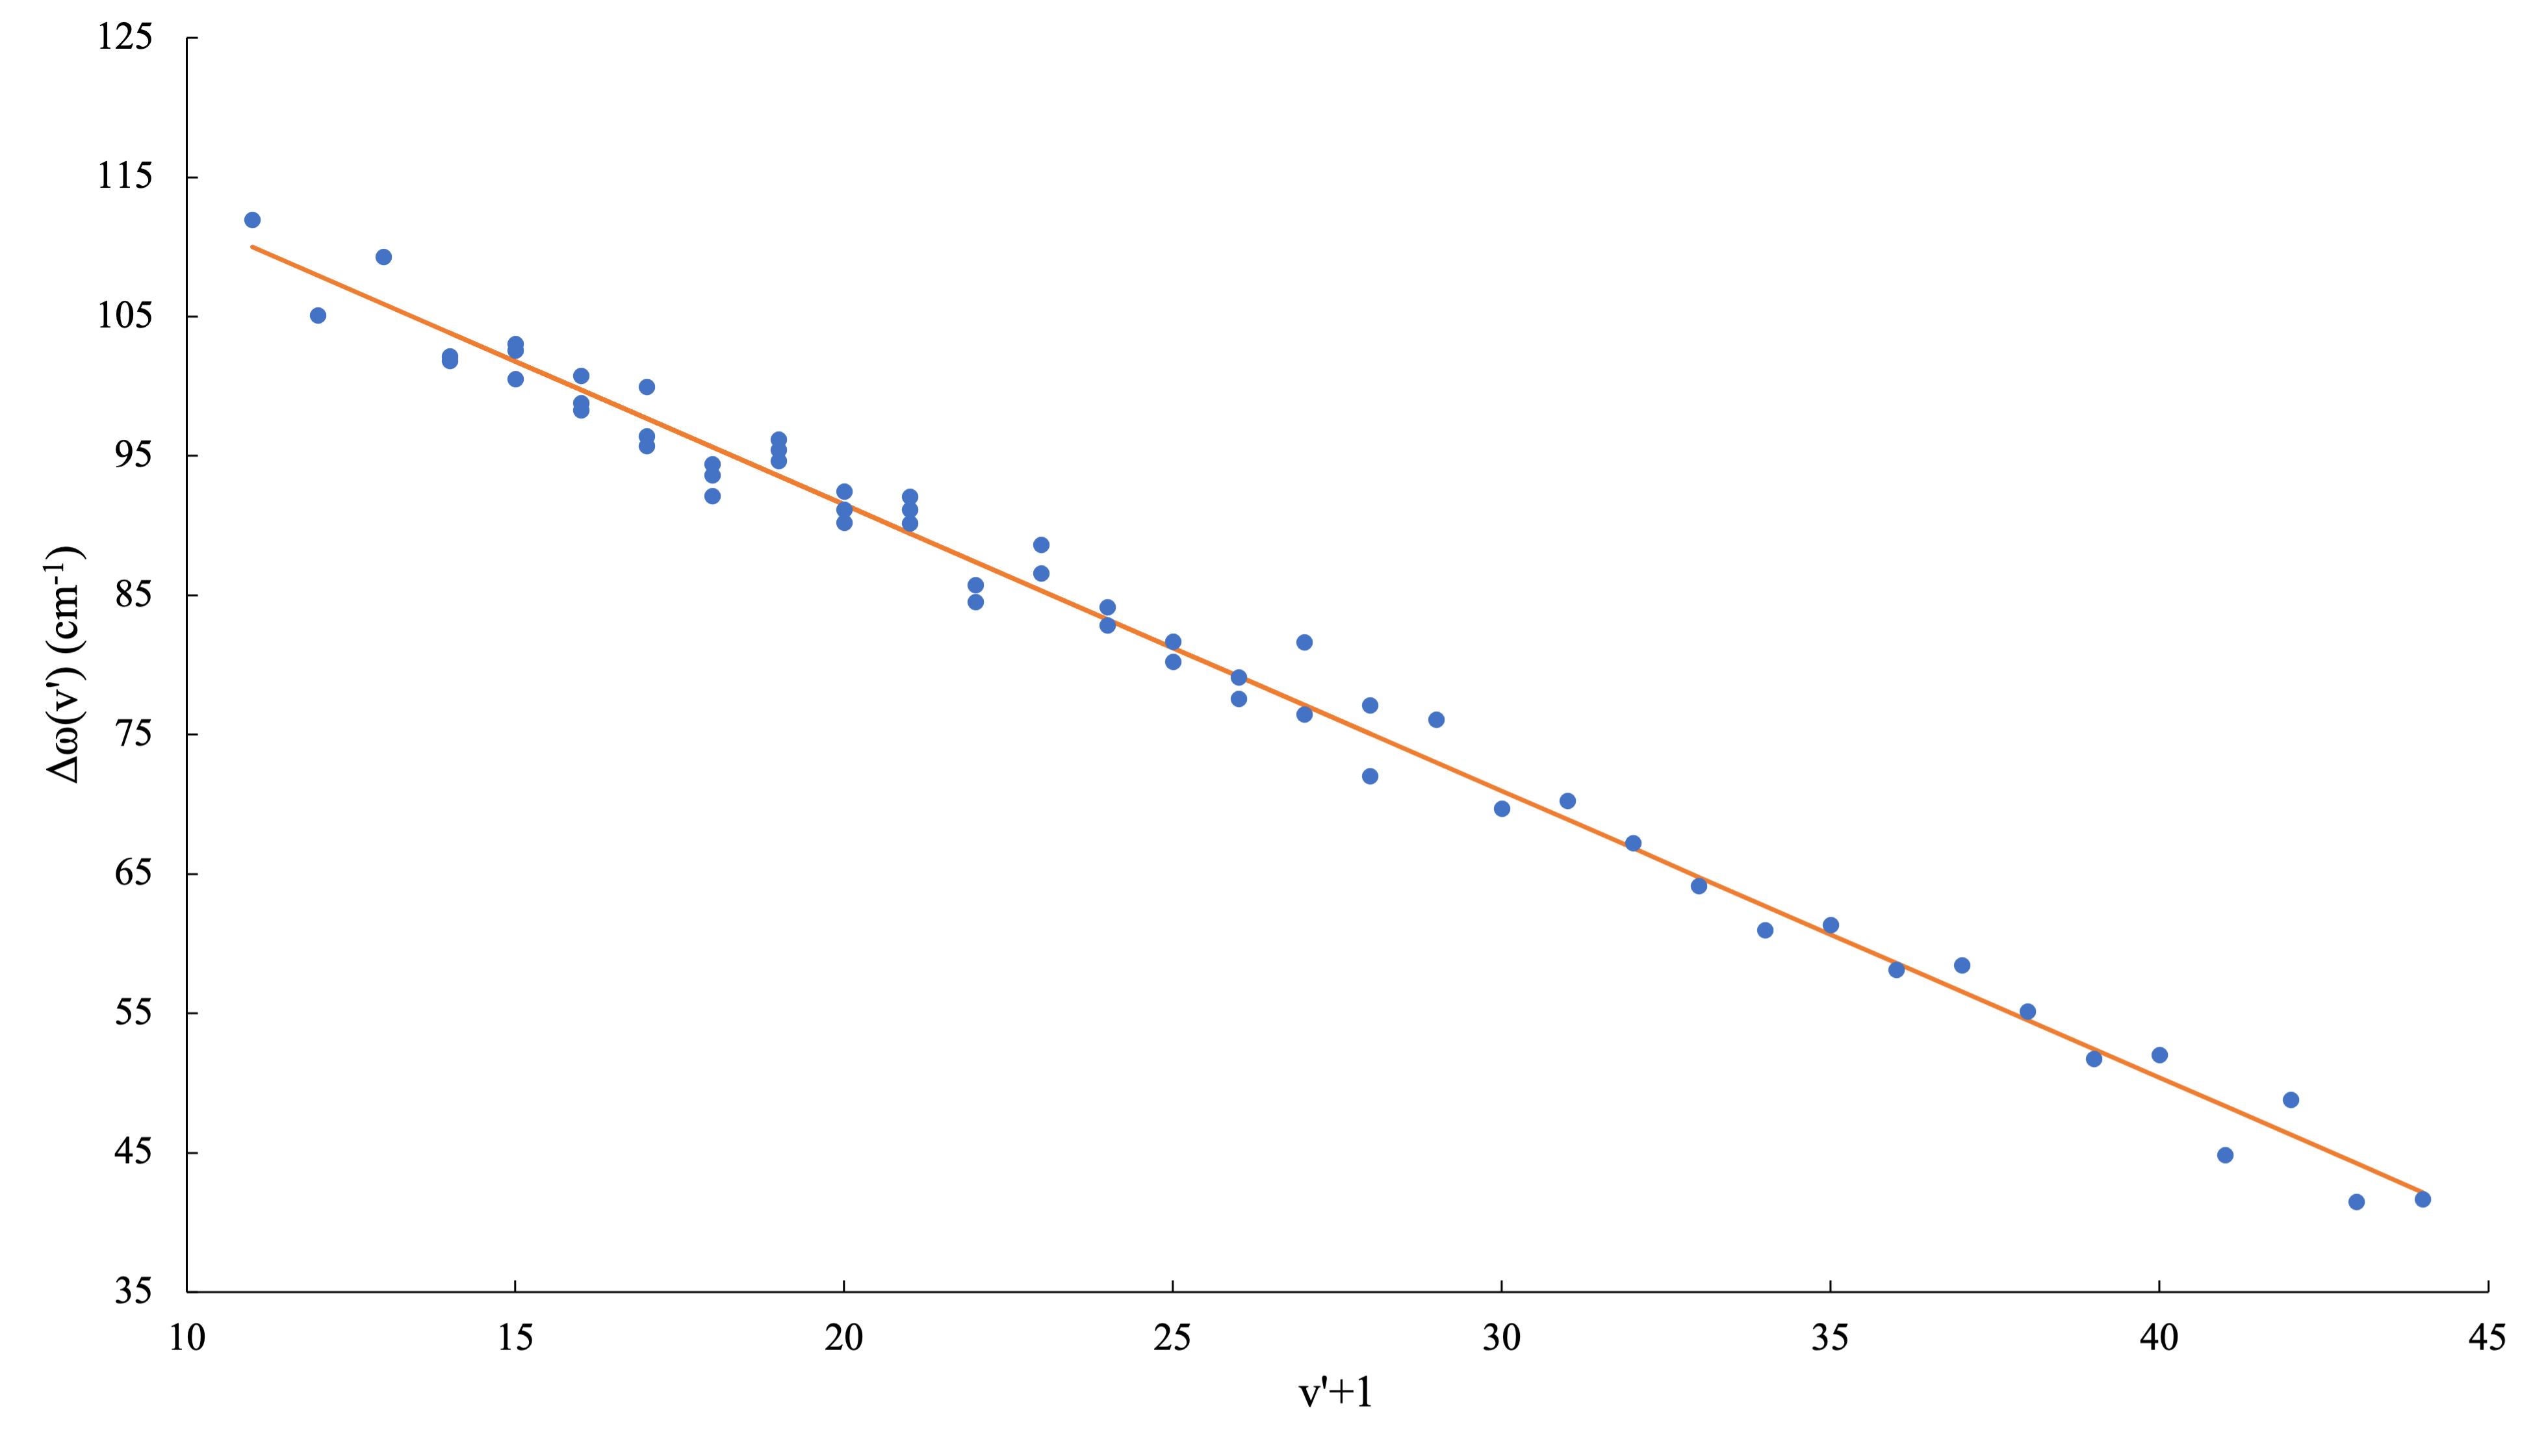
\includegraphics[width=0.95\linewidth]{lab1-BirgeSponerB.png}
    \caption{Birge-Sponer plot for the B state.}
    \label{fig:BirgeSponerB}
\end{figure}

\begin{table}[H]
    \centering
    \small
    \renewcommand{\arraystretch}{1.2}
    \begin{tabular}{|c|c|c|c|c|c|c|c|c|c|}
        \hline
         & $\bm{\bar{\nu}_e'}$ & $\bm{\bar{\nu}_e'x_e'}$ & $\bm{D_e'}$ & $\bm{D_0'}$ & $\bm{\bar{\nu}_e''}$ & $\bm{\bar{\nu}_e''x_e''}$ & $\bm{D_e''}$ & $\bm{D_0''}$ & $\bm{T_e}$\\
        \hline
        \textbf{Calculated values} & \num{132.62} & \num{1.0279} & \num{4277.2} & \num{4211.1} & \num{216.10} & \num{1.2583} & \num{9278.5} & \num{9170.7} & \num{12604}\\
        \hline
        \textbf{Literature values}\supercite{bib:NISTDiatomics}\textsuperscript{,}\supercite{bib:McNaughtI2} & \num{125.69} & \num{0.764} & \num{4112} & \num{4046} & \num{214.50} & \num{0.614} & \num{12244} & \num{12137} & \num{15769.01}\\
        \hline
    \end{tabular}
    \caption{Calculated spectroscopic constants and their reported values.}
    \label{tab:UVVisConstants}
\end{table}
Note that the units for all values in Table \ref{tab:UVVisConstants} is \si{\per\centi\meter}.

\begin{figure}[h!]
    \centering
    \begin{tikzpicture}[
        scale=3,
        every node/.style={black}
    ]
        \small
        \draw (2,2) -- node[rotate=90,above=1cm]{Energy (\si{\per\centi\meter})} (2,0) -- node[below=3mm]{Bond length (\si{\angstrom})} (5,0);

        \footnotesize
        \foreach \x in {2,2.5,...,5} {
            \draw (\x,0.03) -- (\x,0) node[below]{\x};
        }
        \foreach \y/\nam in {0/0,0.5/5000,1/10000,1.5/15000,2/20000} {
            \draw (2.03,\y) -- (2,\y) node[left]{\nam};
        }

        \draw [rex,thick] plot[domain=2.255:5,variable=\r,smooth,samples=100] (\r,{0.92785*(e^(-2.1833*(\r-2.666))-1)^2}) node[above left]{X state};
        \draw [rex,thick] plot[domain=2.77:5,variable=\r,smooth,samples=100] (\r,{0.42772*(e^(-3.2157*(\r-3.024))-1)^2+1.2604}) node[above left]{B state};
    \end{tikzpicture}
    \caption{Morse potential curves.}
    \label{fig:Morse}
\end{figure}

\printbibliography
\setcounter{figure}{0}
\setcounter{table}{0}




\end{document}